% latex foo.tex 
% dvips -Poutline -G0 foo.dvi -o 
% ps2pdf -dPDFSETTINGS#/prepress foo.ps
\documentclass[slidestop,xcolor=pst]{beamer}
\usepackage{etex}
\usepackage{fancyvrb}
\usepackage{hyperref}
%\usepackage{pstricks,pst-tree,pst-node,pst-plot,pst-3dplot}
\usepackage{graphicx}
\usepackage{tikz}
\usetikzlibrary{arrows}

\newcommand{\mygraph}[2]{\includegraphics[width=#1\textwidth]{figures/#2}}
\newcommand{\mygraphc}[2]{\centerline{\includegraphics[width=#1\textwidth]{figures/#2}}}

\newcommand{\sect}[1]{
\section{#1}
\begin{frame}[fragile]\frametitle{#1}
}

\mode<presentation>
{
%  \usetheme{Madrid}
  % or ...

%  \setbeamercovered{transparent}
  % or whatever (possibly just delete it)
}

\usepackage[english]{babel}

\usepackage[latin1]{inputenc}

\title[Computer Graphics, CSCI 480, Ray Tracing IV]
{
Ray Tracing, Part IV
}

\subtitle{} % (optional)

\author[Geoffrey Matthews]
{Geoffrey Matthews}
% - Use the \inst{?} command only if the authors have different
%   affiliation.

\institute[WWU/CS]
{
  Department of Computer Science\\
  Western Washington University
}
% - Use the \inst command only if there are several affiliations.
% - Keep it simple, no one is interested in your street address.

\date{Fall 2015}

% If you have a file called "university-logo-filename.xxx", where xxx
% is a graphic format that can be processed by latex or pdflatex,
% resp., then you can add a logo as follows:

%\pgfdeclareimage[height=0.5cm]{university-logo}{WWULogoProColor}
%\logo{\pgfuseimage{university-logo}}

% If you wish to uncover everything in a step-wise fashion, uncomment
% the following command: 

%\beamerdefaultoverlayspecification{<+->}

\newcommand{\bi}{\begin{itemize}}
\newcommand{\ei}{\end{itemize}}
\newcommand{\myref}[1]{\small\item\url{#1}}
\newcommand{\myreff}[1]{\scriptsize\item\url{#1}}

\begin{document}


\begin{frame}
  \titlepage
\end{frame}

\sect{Readings}
\bi
\item\url{https://en.wikipedia.org/wiki/Gradient}
\item  \url{https://en.wikipedia.org/wiki/Quadric}
\item\url{http://www.win.tue.nl/~sterk/Bouwkunde/hoofdstuk3.pdf}
\ei
\end{frame}

\sect{Ellipsoids}
\begin{columns}
  \begin{column}{0.5\textwidth}
\mygraphc{0.6}{Ellipsoid_Quadric.png}
  \end{column}
  \begin{column}[b]{0.5\textwidth}
\[
\frac{x^2}{a^2} + \frac{y^2}{b^2} + \frac{z^2}{c^2} = 1
\]
  \end{column}
\end{columns}

\vfill

\bi
\item How can we intersect a ray with this surface?
\item How can we find the normal?
\item How can we rotate this shape?
\ei
\end{frame}


\sect{Intersect a ray with an ellipsoid}
Constraint on the surface:
\[
\frac{x^2}{a^2} + \frac{y^2}{b^2} + \frac{z^2}{c^2} = 1
\]
Points on the line generated by:
\[
p + tv = (p_0,p_1,p_2) + t(v_0,v_1,v_2)
\]
Plug one into the other to satisfy both:
\[
\frac{(p_0+tv_0)^2}{a^2} + \frac{(p_1+tv_1)^2}{b^2} + \frac{(p_2+tv_2)^2}{c^2} = 1
\]
Collect terms to get our quadratic to solve:
\[
\left(\frac{v_0^2}{a^2} + \frac{v_1^2}{b^2} +
\frac{v_2^2}{c^2}\right)t^2
+
\left(\frac{2p_0v_0}{a^2} + \frac{2p_1v_1}{b^2} +
\frac{2p_2v_2}{c^2}\right)t
+
\left(\frac{p_0^2}{a^2} + \frac{p_1^2}{b^2} +
\frac{p_2^2}{c^2}\right)
\]
\end{frame}

\sect{How do we move ellipsoids away from the origin?}
\mygraphc{0.7}{randomellipsoids03.png}
\end{frame}

\sect{What about the normal for an ellipsoid?}
\mygraphc{0.7}{randomellipsoids02.png}
\end{frame}

\sect{Calculus to the rescue!}
\bi
\item
Ellipsoids satisfy the constraint:
\[
f(x,y,z) = \frac{x^2}{a^2} + \frac{y^2}{b^2} + \frac{z^2}{c^2} = 1
\]
\item
This means that the function $f$ is {\em constant} across the
surface.  If we take the {\em gradient} of $f$, it will be a vector pointing
in the direction of maximum change of $f$, which will be perpendicular
to the directions in which it is not changing at all.
\item
  The gradient is defined as
\[
\nabla f(x,y,z) = \left(
\frac{\partial f}{\partial x} ,
\frac{\partial f}{\partial y} ,
\frac{\partial f}{\partial z}
\right)
\]
\item
The partial derivative of a function, for example, $\frac{\partial
  f}{\partial x}$, is simply the derivative of $f$ treating everything
except $x$ as a constant.
\ei
\end{frame}

\sect{Normals for the ellipsoid}
\bi
\item For the ellipsoid, the function is
\[
f(x,y,z) = \frac{x^2}{a^2} + \frac{y^2}{b^2} + \frac{z^2}{c^2}
\]
\item What is the gradient of this function? \pause
\[
\nabla f(x,y,z) = \left(\frac{2x}{a^2} , \frac{2y}{b^2} , \frac{2z}{c^2}\right)
\]
\item Since we want to normalize this anyway, we can drop the factor of 2.
\item
Note that this is in coordinates where the ellipsoid has not been
translated.  After we find our translated intersection point, we have
to translate it back by subtracting the ellipsoid's center before
calculating the normal.
\item Or just use the translated ray to find the $(x,y,z)$ for the
  gradient while calculating the intersection.  
\ei
\end{frame}

\sect{Can use ellipsoids for lots of things}
\mygraphc{0.7}{axesworld.png}
\end{frame}

\sect{Other quadrics}
\bi
\item Using the tips above for the ellipsoid, you should be able to
  render any of the quadrics from this page:
  \url{https://en.wikipedia.org/wiki/Quadric}
  \ei
\end{frame}

\sect{Rotating ellipsoids}
\mygraphc{0.7}{ellipsoidworld.png}
\end{frame}

\sect{How do we rotate quadrics?}
\mygraphc{0.7}{rotatedellipsoids.png}
\end{frame}

\sect{Rotating points}
\begin{columns}
  \column{0.5\textwidth}
  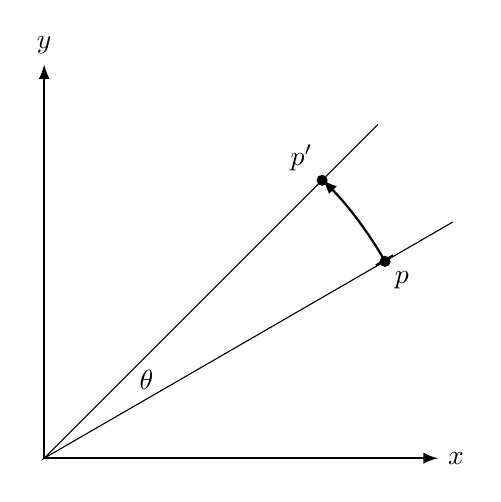
\begin{tikzpicture}[>=latex,baseline=(current bounding box.north)]
    %\draw[help lines] (-1,-1) grid (6,6);
    \draw[<->,thick] (5,0) node[anchor=west] {$x$}-- (0,0) -- (0,5) node[anchor=south] {$y$};
    \draw (5.19,3) -- (0,0) -- (4.24,4.24);
    \fill (4.33,2.5) circle (2pt) node[anchor=north west] {$p$};
    \fill (3.53,3.53) circle (2pt) node[anchor=south east] {$p'$};
    \draw[|->,thick] (30:5) arc (30:45:5);
    \draw (1.3,1) node {$\theta$};
  \end{tikzpicture}
  \column{0.5\textwidth}
  \begin{eqnarray*}
    x' &=& x\cos(\theta) - y\sin(\theta)\\
    y' &=& x\sin(\theta) + y\cos(\theta)
  \end{eqnarray*}
  \pause
  \begin{itemize}
    \item What if we want to rotate in the opposite direction? \pause
  \item If $z$ is pointing in, is this a
    \begin{itemize}
    \item right-handed frame?
    \item right-handed rotation?
    \end{itemize}
    \pause
  \item What about $z$ pointing out?
    \pause
  \item What about rotating vectors?
    \pause
  \end{itemize}
\end{columns}

\vfill
For derivation of equation:
\url{https://engineering.purdue.edu/~bethel/rot2.pdf}

\end{frame}

\sect{Rotating in 3D}
\bi
\item Rotating around the $z$ axis:
  \[
  p' = (x\cos(\theta) - y\sin(\theta), x\sin(\theta) + y\cos(\theta), z)
  \]
\item Rotating around the $y$ axis:
  \[
  p' = (x\cos(\theta) - z\sin(\theta), y, x\sin(\theta) + z\cos(\theta))
  \]
\item Rotating around the $x$ axis:
  \[
  p' = (x, y\cos(\theta) - z\sin(\theta), y\sin(\theta) + z\cos(\theta))
  \]
\item General rotations can be built up as sequences of $x$, $y$ and
  $z$ rotations.
  \ei
\end{frame}

\sect{Rotating quadrics}
\mygraphc{0.7}{rotatedellipsoids02.png}
\end{frame}

\sect{Rotating quadrics}
\mygraphc{0.7}{ellipsoidworld.png}
\end{frame}


\sect{What about rotating quadrics?}
\begin{tikzpicture}
%  \draw[help lines] (0,0) grid (10,2);
  \draw[thick] (8,0) -- (8,2) -- (10,2) -- (10,0) -- (8,0);
\draw[thick,gray,|->] (10.5,1) arc [radius=1.5, start angle=0, end angle=30];
  \draw[thick,*->] (0,1) -- (2,1);
\draw[thick,blue] (8.63, -0.37) -- (7.63, 1.37) -- (9.37, 2.37) -- (10.37, 0.63) -- cycle;
\end{tikzpicture}

\pause
\vfill
\hrulefill
\vfill

\begin{tikzpicture}
%\draw[help lines] (0,0) grid (10,4);
  \draw[thick] (8,0) -- (8,2) -- (10,2) -- (10,0) -- (8,0);
  \draw[thick,*->] (0,1) -- (2,1);
  \draw[thick,gray,|->] (-0.2,1) arc [radius=9.2, start angle=180, end angle=160];
  \draw[thick,red,*->] (0.5,4) -- (2.5,3.28);
\end{tikzpicture}

\end{frame}

\sect{How do we find the intersection point?}

\begin{tikzpicture}
%\draw[help lines] (0,0) grid (10,4);
  \draw[thick] (8,0) -- (8,2) -- (10,2) -- (10,0) -- (8,0);
  \draw[thick,*->] (0,1) -- (2,1);
  \draw[thick,gray,|->] (-0.2,1) arc [radius=9.2, start angle=180, end angle=160];
  \draw[thick,red,*->] (0.5,4) -- (2.5,3.28);
  \draw[dotted,red] (0.5,4) -- (9,1);
  \fill[red] (8,1.328) circle (2pt);
\draw[thick,blue] (8.63, -0.37) -- (7.63, 1.37) -- (9.37, 2.37) -- (10.37, 0.63) -- cycle;
\draw[dotted,blue] (0,1) -- (9,1);
\draw[thick,gray,|->] (10.5,1) arc [radius=1.5, start angle=0, end angle=30];
  \fill[blue] (7.85,1) circle (2pt);
\end{tikzpicture}

\pause
\begin{itemize}
\item Translate the ray point (subtract the object center).
\item Rotate the ray point by the {\em inverse} rotation of the object.
\item Rotate the ray vector by the {\em inverse} rotation of the object.
\item Find $t$, the distance along the ray to the intersection.
\item Use $t$ with the original ray to find the point in world coordinates. 
\end{itemize}

\end{frame}

\sect{How do we find the normal?}


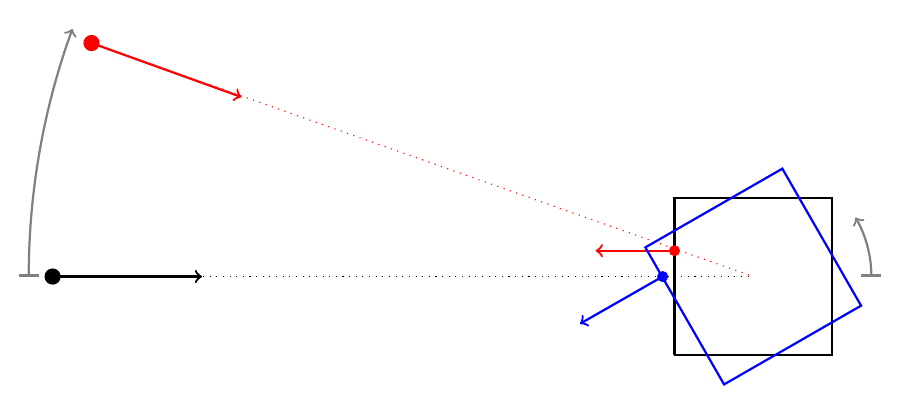
\begin{tikzpicture}
%\draw[help lines] (0,0) grid (10,4);
  \draw[thick] (8,0) -- (8,2) -- (10,2) -- (10,0) -- (8,0);
  \draw[thick,*->] (0,1) -- (2,1);
  \draw[thick,gray,|->] (-0.2,1) arc [radius=9.2, start angle=180, end angle=160];
  \draw[thick,red,*->] (0.5,4) -- (2.5,3.28);
  \draw[dotted,red] (0.5,4) -- (9,1);
  \fill[red] (8,1.328) circle (2pt);
\draw[red,->,thick] (8,1.328) -- (7,1.328);
\draw[thick,blue] (8.63, -0.37) -- (7.63, 1.37) -- (9.37, 2.37) -- (10.37, 0.63) -- cycle;
\draw[thick,gray,|->] (10.5,1) arc [radius=1.5, start angle=0, end angle=30];
  \fill[blue] (7.85,1) circle (2pt);
\draw[blue,->,thick] (7.85,1) -- (6.8, .4);
\draw[dotted] (1,1) -- (9,1);
\end{tikzpicture}


\pause
\begin{itemize}
\item Translate and rotate the ray to find the hit point.
  \item Use the {\em inverse} rotation of the object to rotate the ray.
  \item Find the normal at the hit point.\\Use the gradient as the quadric is untransformed.
\item Rotate this normal using the {\em original} rotation matrix.
\end{itemize}


\end{frame}

\sect{Putting it all together}
\mygraphc{0.7}{randomellipsoids.png}
\end{frame}

\end{document}

